\documentclass[tikz,border=4pt]{standalone}
\usepackage{amsmath}
\begin{document}
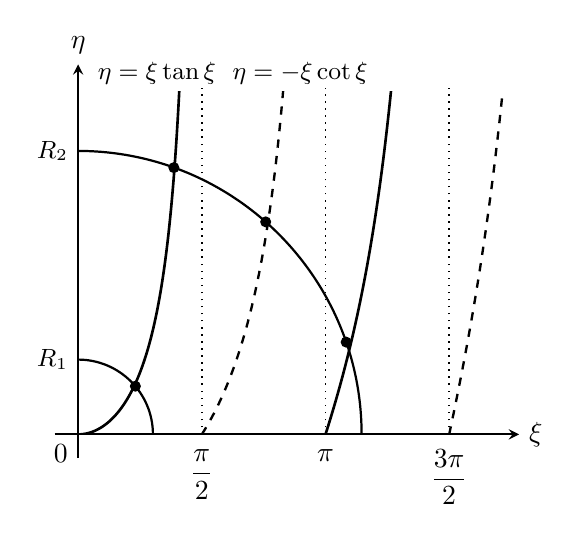
\begin{tikzpicture}[>=stealth, thick, scale=1.0]
  % Axes: xi horizontal (0 to 5.5), eta vertical (0 to 4.8)
  % Unit scale: 1 rad = 1.0 cm
  \draw[->, line width=0.65pt] (-0.3, 0) -- (5.6, 0) node[right] {$\xi$};
  \draw[->, line width=0.65pt] (0, -0.3) -- (0, 4.7) node[above] {$\eta$};
  \node[below left] at (0, 0) {$0$};

  % Vertical asymptotes at pi/2 (~1.571), pi (~3.142), 3pi/2 (~4.712)
  \draw[dotted, line width=0.55pt] (1.571, 0) -- (1.571, 4.4);
  \draw[dotted, line width=0.55pt] (3.142, 0) -- (3.142, 4.4);
  \draw[dotted, line width=0.55pt] (4.712, 0) -- (4.712, 4.4);

  \node[below] at (1.571, -0.06) {$\dfrac{\pi}{2}$};
  \node[below] at (3.142, -0.06) {$\pi$};
  \node[below] at (4.712, -0.06) {$\dfrac{3\pi}{2}$};

  % Clip curves to plot box
  \begin{scope}
    \clip (0, 0) rectangle (5.4, 4.35);

    % Even parity: eta = xi * tan(xi) (solid)
    \draw[line width=0.95pt, domain=0:1.30, samples=80, smooth] plot (\x, {\x * tan(\x r)});
    \draw[line width=0.95pt, domain=3.142:4.16, samples=80, smooth] plot (\x, {\x * tan(\x r)});

    % Odd parity: eta = -xi * cot(xi) (dashed)
    \draw[line width=0.85pt, dashed, domain=1.571:2.64, samples=80, smooth] plot (\x, {-\x / tan(\x r)});
    \draw[line width=0.85pt, dashed, domain=4.712:5.40, samples=60, smooth] plot (\x, {-\x / tan(\x r)});

    % Small circle R1 = 0.95 (shallow well: 1 even bound state only)
    \draw[line width=0.8pt] (0.95, 0) arc (0:90:0.95);
    % Larger circle R2 = 3.6 (multiple bound states)
    \draw[line width=0.8pt] (3.6, 0) arc (0:90:3.6);
  \end{scope}

  % Intersection points for R1 = 0.95 (xi ~ 0.727, eta ~ 0.612)
  \fill (0.727, 0.612) circle (2.0pt);
  % Intersection points for R2 = 3.6:
  % Even 1: xi ~ 1.216, eta ~ 3.388
  % Odd 1: xi ~ 2.382, eta ~ 2.699
  % Even 2: xi ~ 3.404, eta ~ 1.172
  \fill (1.216, 3.388) circle (2.0pt);
  \fill (2.382, 2.699) circle (2.0pt);
  \fill (3.404, 1.172) circle (2.0pt);

  % Curve labels placed cleanly above the clipped curves
  \node[font=\small] at (1.00, 4.58) {$\eta = \xi\tan\xi$};
  \node[font=\small] at (2.82, 4.58) {$\eta = -\xi\cot\xi$};

  % Circle radius labels
  \node[font=\small, left] at (0.0, 0.95) {$R_1$};
  \node[font=\small, left] at (0.0, 3.60) {$R_2$};
\end{tikzpicture}
\end{document}
